\documentclass[11pt]{article}
\usepackage[textwidth=18.0cm, textheight=23.0cm, top=2.0cm]{geometry}
\usepackage{pst-all}
\usepackage{amssymb}
\usepackage{tikz}
\usepackage{underscore}\begin{document}
\pagestyle{empty}


ClassName: \underline{\textbf{Class_07.2bp-2}}
\par
BinSize: \underline{\textbf{100 × 100}}
\par
ReduceSize: \underline{\textbf{100 × 100}}
\par
TypeNum: \underline{\textbf{20}}
\par
Num: \underline{\textbf{20}}
\par
OutS: \underline{\textbf{50000}}
\par
InS: \underline{\textbf{39269}}
\par
Rate: \underline{\textbf{0.785}}
\par
UB: \underline{\textbf{5}}
\par
LB0: \underline{\textbf{5}}
\par
LB: \underline{\textbf{5}}
\par
LBWithCut: \underline{\textbf{5}}
\par
NodeCut: \underline{\textbf{0}}
\par
ExtendedNodeCnt: \underline{\textbf{1}}
\par
GenNodeCnt: \underline{\textbf{1}}
\par
PrimalNode: \underline{\textbf{0}}
\par
ColumnCount: \underline{\textbf{5}}
\par
TotalCutCount: \underline{\textbf{0}}
\par
RootCutCount: \underline{\textbf{0}}
\par
LPSolverCnt: \underline{\textbf{1}}
\par
PricingSolverCnt: \underline{\textbf{0}}
\par
BranchAndBoundNum: \underline{\textbf{1}}
\par
isOpt: \underline{\textbf{true}}
\par
TimeOnPrimal: \underline{\textbf{0.000 s}}
\par
TimeOnPricing: \underline{\textbf{0.000 s}}
\par
TimeOnRmp: \underline{\textbf{0.063 s}}
\par
TotalTime: \underline{\textbf{0.110 s}}
\par
\newpage


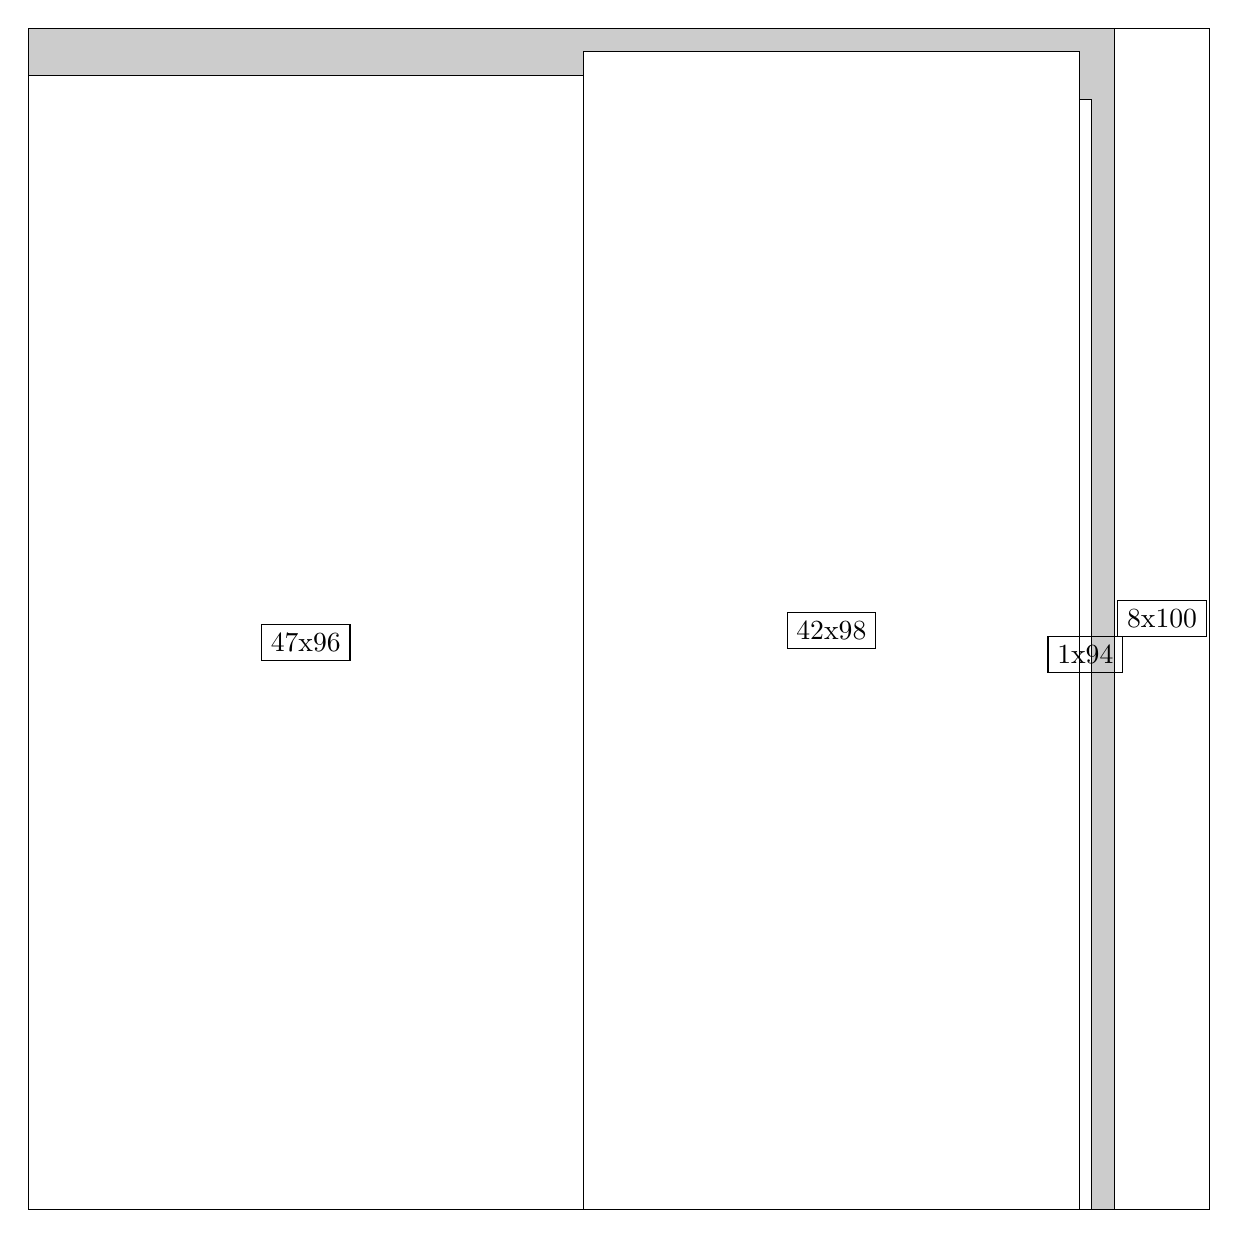
\begin{tikzpicture}[shorten >=1pt,scale=1.0,every node/.style={scale=1.0},->]
\tikzstyle{vertex}=[circle,fill=black!25,minimum size=14pt,inner sep=0pt]
\filldraw[fill=gray!40!white, draw=black] (0,0) rectangle (15.0,15.0);
\foreach \name/\x/\y/\w/\h in {47x96/0.0/0.0/7.05/14.399999999999999,42x98/7.05/0.0/6.3/14.7,8x100/13.799999999999999/0.0/1.2/15.0,1x94/13.35/0.0/0.15/14.1}
\filldraw[fill=white!40!white, draw=black] (\x,\y) rectangle node[draw] (\name) {\name} ++(\w,\h);
\end{tikzpicture}


w =47 , h =96 , x =0 , y =0 , v =4512
\par
w =42 , h =98 , x =47 , y =0 , v =4116
\par
w =8 , h =100 , x =92 , y =0 , v =800
\par
w =1 , h =94 , x =89 , y =0 , v =94
\par
\newpage


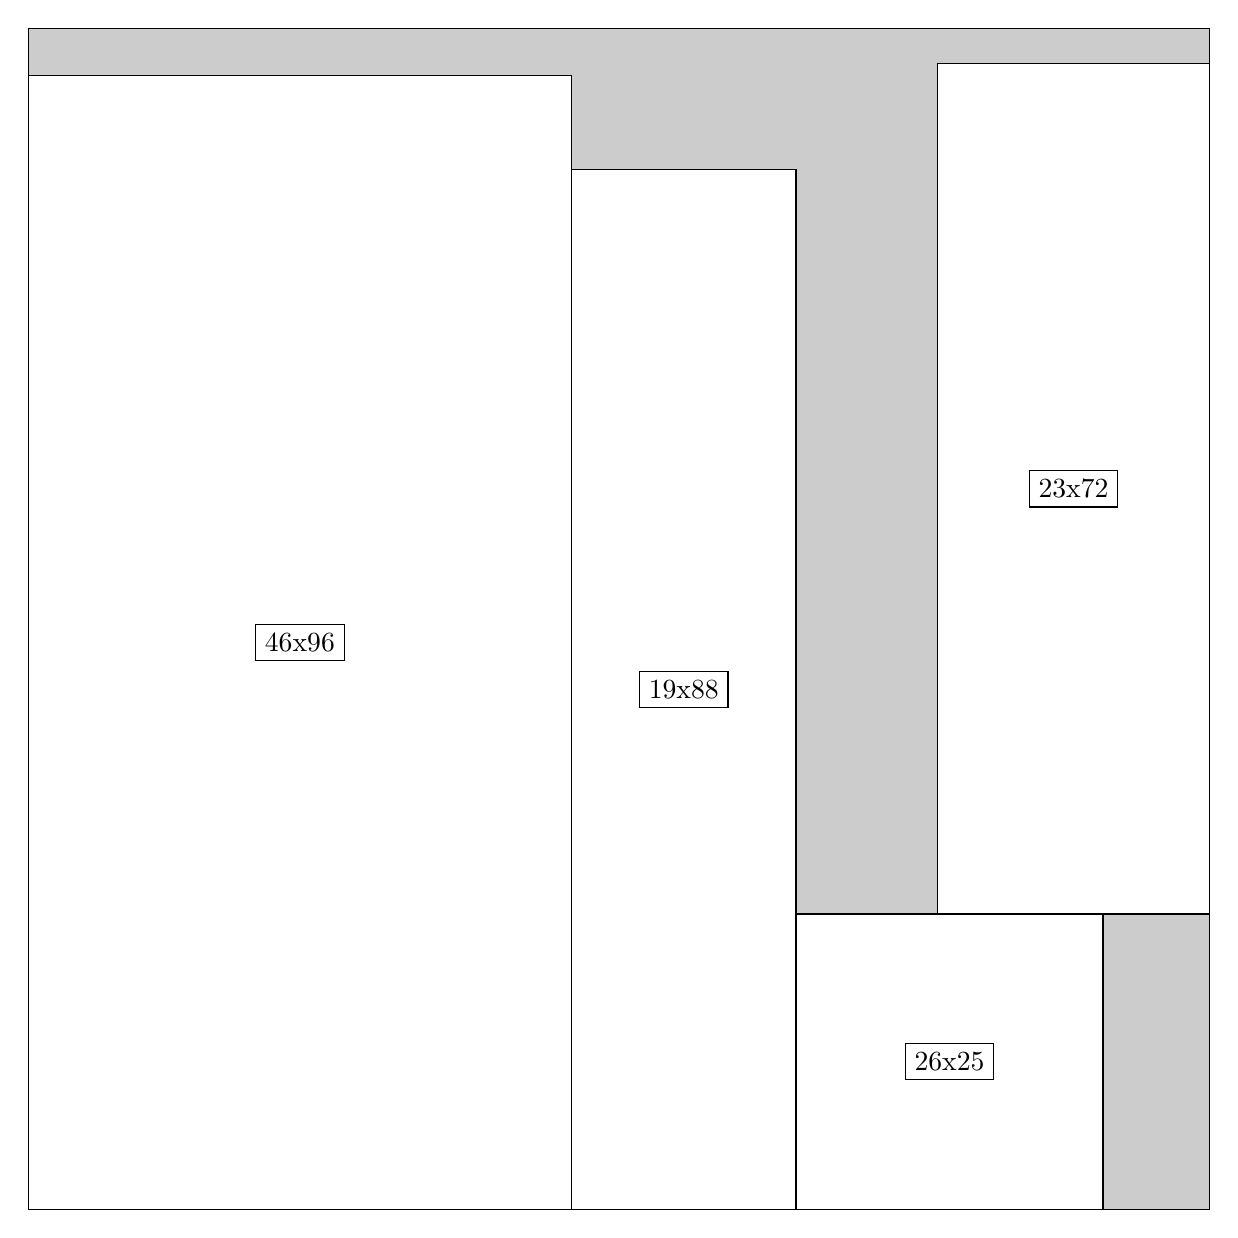
\begin{tikzpicture}[shorten >=1pt,scale=1.0,every node/.style={scale=1.0},->]
\tikzstyle{vertex}=[circle,fill=black!25,minimum size=14pt,inner sep=0pt]
\filldraw[fill=gray!40!white, draw=black] (0,0) rectangle (15.0,15.0);
\foreach \name/\x/\y/\w/\h in {46x96/0.0/0.0/6.8999999999999995/14.399999999999999,19x88/6.8999999999999995/0.0/2.85/13.2,23x72/11.549999999999999/3.75/3.4499999999999997/10.799999999999999,26x25/9.75/0.0/3.9/3.75}
\filldraw[fill=white!40!white, draw=black] (\x,\y) rectangle node[draw] (\name) {\name} ++(\w,\h);
\end{tikzpicture}


w =46 , h =96 , x =0 , y =0 , v =4416
\par
w =19 , h =88 , x =46 , y =0 , v =1672
\par
w =23 , h =72 , x =77 , y =25 , v =1656
\par
w =26 , h =25 , x =65 , y =0 , v =650
\par
\newpage


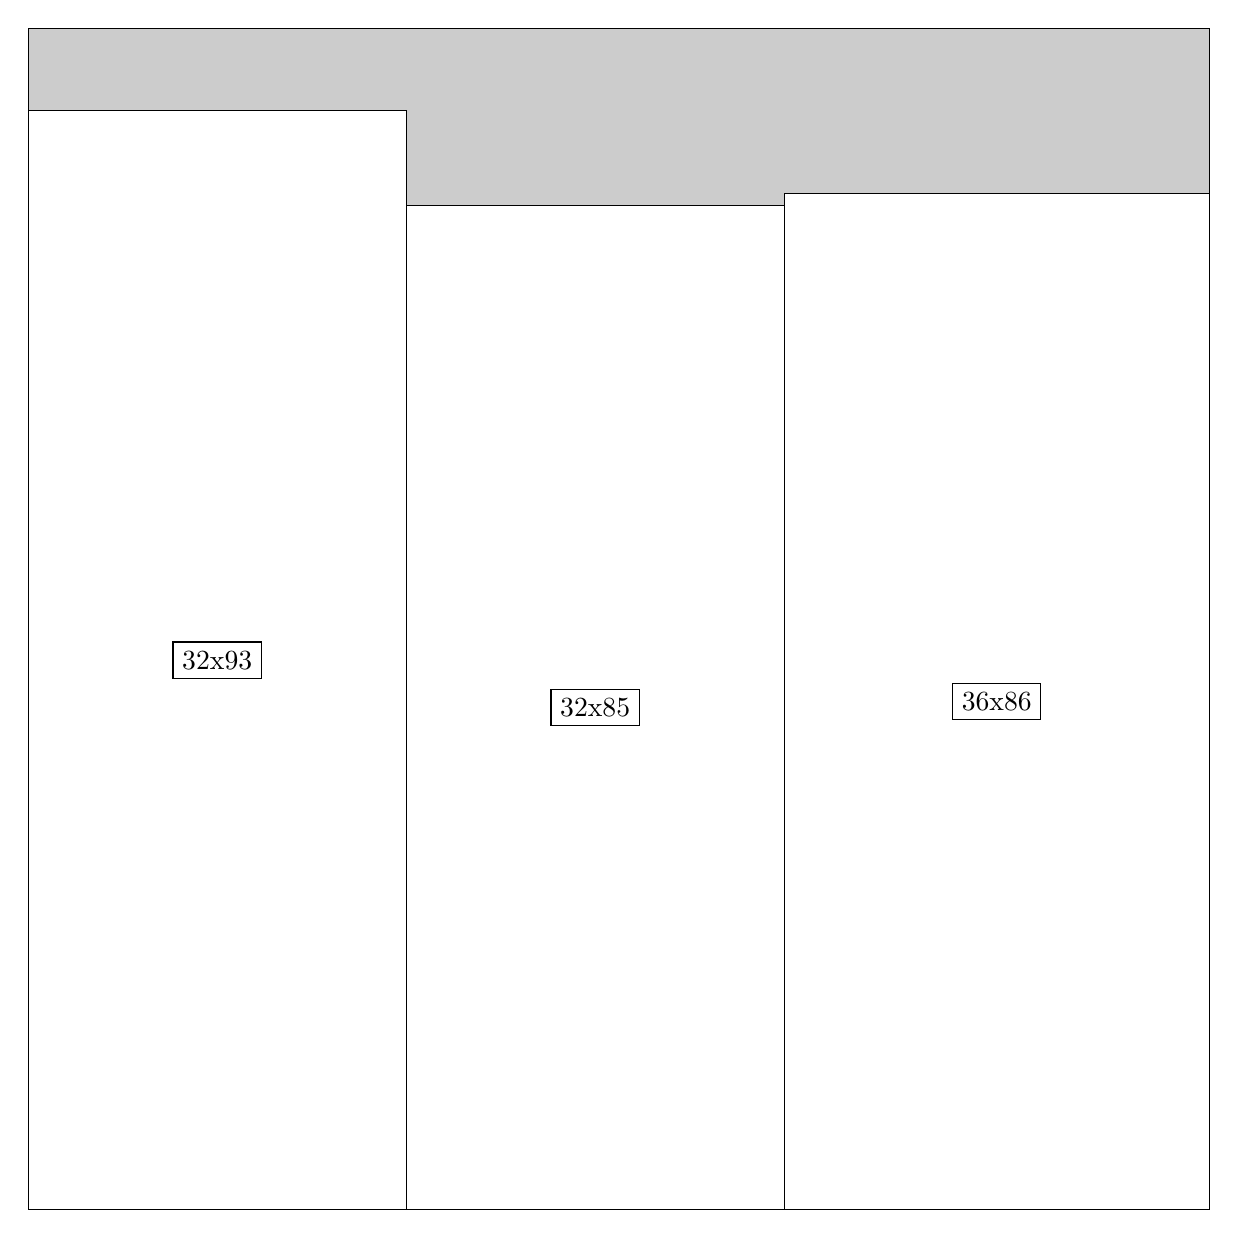
\begin{tikzpicture}[shorten >=1pt,scale=1.0,every node/.style={scale=1.0},->]
\tikzstyle{vertex}=[circle,fill=black!25,minimum size=14pt,inner sep=0pt]
\filldraw[fill=gray!40!white, draw=black] (0,0) rectangle (15.0,15.0);
\foreach \name/\x/\y/\w/\h in {32x93/0.0/0.0/4.8/13.95,32x85/4.8/0.0/4.8/12.75,36x86/9.6/0.0/5.3999999999999995/12.9}
\filldraw[fill=white!40!white, draw=black] (\x,\y) rectangle node[draw] (\name) {\name} ++(\w,\h);
\end{tikzpicture}


w =32 , h =93 , x =0 , y =0 , v =2976
\par
w =32 , h =85 , x =32 , y =0 , v =2720
\par
w =36 , h =86 , x =64 , y =0 , v =3096
\par
\newpage


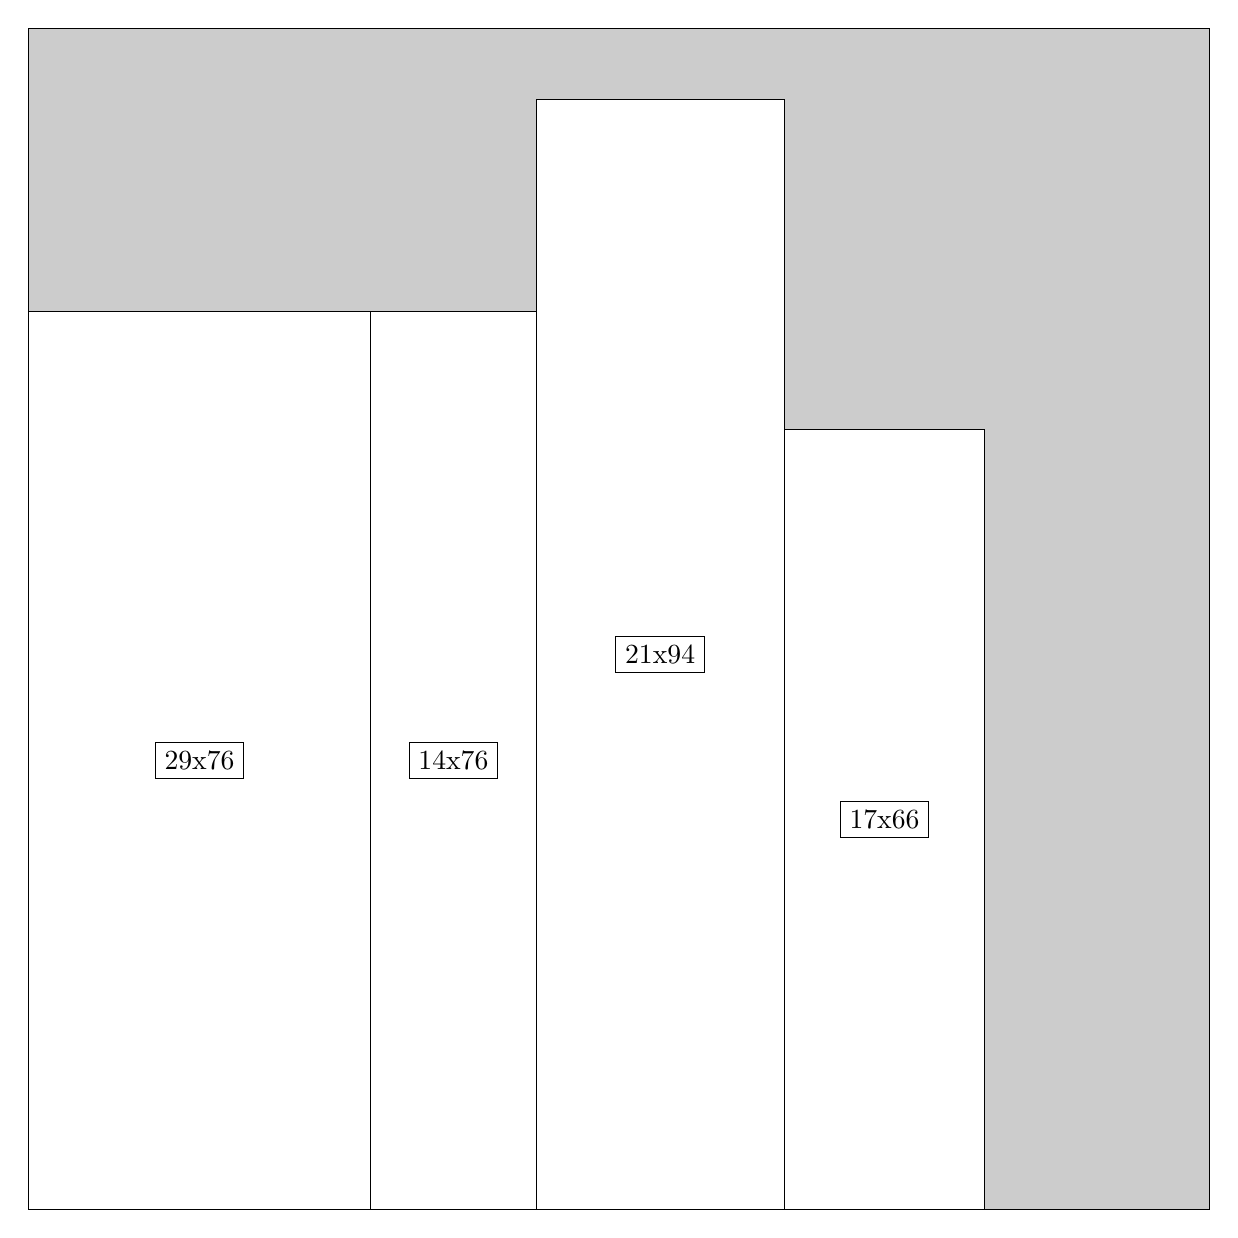
\begin{tikzpicture}[shorten >=1pt,scale=1.0,every node/.style={scale=1.0},->]
\tikzstyle{vertex}=[circle,fill=black!25,minimum size=14pt,inner sep=0pt]
\filldraw[fill=gray!40!white, draw=black] (0,0) rectangle (15.0,15.0);
\foreach \name/\x/\y/\w/\h in {29x76/0.0/0.0/4.35/11.4,21x94/6.45/0.0/3.15/14.1,17x66/9.6/0.0/2.55/9.9,14x76/4.35/0.0/2.1/11.4}
\filldraw[fill=white!40!white, draw=black] (\x,\y) rectangle node[draw] (\name) {\name} ++(\w,\h);
\end{tikzpicture}


w =29 , h =76 , x =0 , y =0 , v =2204
\par
w =21 , h =94 , x =43 , y =0 , v =1974
\par
w =17 , h =66 , x =64 , y =0 , v =1122
\par
w =14 , h =76 , x =29 , y =0 , v =1064
\par
\newpage


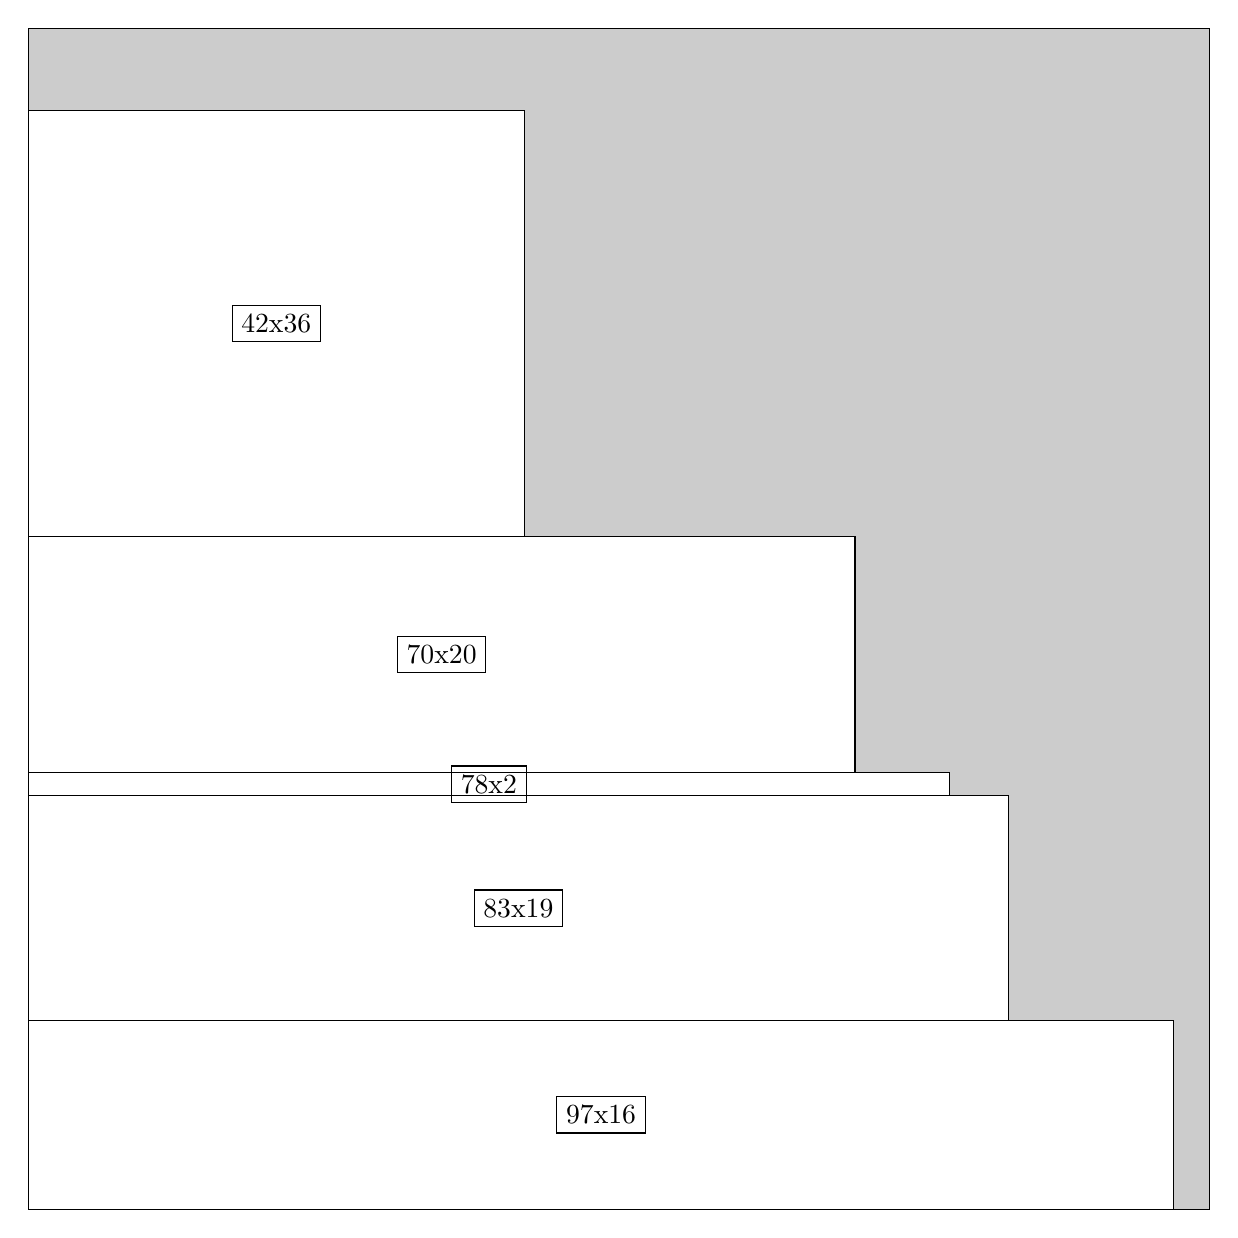
\begin{tikzpicture}[shorten >=1pt,scale=1.0,every node/.style={scale=1.0},->]
\tikzstyle{vertex}=[circle,fill=black!25,minimum size=14pt,inner sep=0pt]
\filldraw[fill=gray!40!white, draw=black] (0,0) rectangle (15.0,15.0);
\foreach \name/\x/\y/\w/\h in {83x19/0.0/2.4/12.45/2.85,97x16/0.0/0.0/14.549999999999999/2.4,42x36/0.0/8.549999999999999/6.3/5.3999999999999995,70x20/0.0/5.55/10.5/3.0,78x2/0.0/5.25/11.7/0.3}
\filldraw[fill=white!40!white, draw=black] (\x,\y) rectangle node[draw] (\name) {\name} ++(\w,\h);
\end{tikzpicture}


w =83 , h =19 , x =0 , y =16 , v =1577
\par
w =97 , h =16 , x =0 , y =0 , v =1552
\par
w =42 , h =36 , x =0 , y =57 , v =1512
\par
w =70 , h =20 , x =0 , y =37 , v =1400
\par
w =78 , h =2 , x =0 , y =35 , v =156
\par
\newpage


\end{document}